%\documentclass[journal]{new-aiaa}
\documentclass[conf]{new-aiaa} %for conference papers
\usepackage{amsmath}
\usepackage{booktabs}
\usepackage{graphicx}
\usepackage[utf8]{inputenc}
\usepackage{lipsum}
\usepackage[version=4]{mhchem}
\usepackage{placeins}
\usepackage{siunitx}
\usepackage{subfig}
\usepackage{siunitx}
\usepackage{textcomp}
\usepackage{longtable,tabularx}

\setlength\LTleft{0pt} 

\title{Online Adaptive Helicopter Control Using Incremental Dual Heuristic Programming}

\author{Bart Helder\footnote{MSc. Student, Control \& Simulation, Faculty of Aerospace Engineering, Delft University of Technology}}
\affil{Delft University of Technology, The Netherlands}  

\begin{document}

\maketitle

\begin{abstract}
Reinforcement learning is an appealing approach for adaptive, fault-tolerant flight control, but is generally plagued by its need for accurate system models and lengthy offline training phases. The novel Incremental Dual Heuristic Programming (IDHP) method removes these dependencies by using an online-identified local system model. A recent implementation has shown to be capable of reliably learning near-optimal control policies for a fixed-wing aircraft in cruise by using outer loop PID and inner-loop IDHP rate controllers. However, fixed-wing aircraft are inherently stable, enabling a trade-off between learning speed and learning stability which is not trivially extended to a physically unstable system. This paper presents an implementation of IDHP for control of a non-linear, six-degree-of-freedom simulation of an MBB Bo-105 helicopter. The proposed system uses two separate IDHP controllers for direct pitch angle and altitude control combined with outer loop and lateral PID controllers. After a short online training phase, the agent is shown to be able to fly a modified ADS-33 acceleration-deceleration manoeuvre as well as a one-engine-inoperative continued landing with high success rates. 
\end{abstract}

\section*{Nomenclature}

%\noindent(Nomenclature entries should have the units identified)

{\renewcommand\arraystretch{1.0}
\noindent\begin{longtable*}{@{}l @{\quad=\quad} l@{}}
% Latin alphabet
$a_t$               & Action taken based on the information of state $s_t$ \\
$e_a, e_c$          & Actor and critic error \\
$F_t, G_t$          & State and control matrix of recursive least squares estimator \\
$L_A, L_C$          & Actor and critic loss \\ 
$n, m$              & Number of states, number of actions\\
$\hat{P}_t$         & Covariance matrix of recursive least squares estimator \\
$P, Q$              & State-selection and weighting matrices \\
$p, q, r$           & Aircraft body rotational rates \\
$r_{t}$             & Reward obtained from transition to state $s_t$ \\
$s_t, s^r_t$        & State and reference state \\
$u, v, w$           & Aircraft body velocities \\
$V(s) $             & State value function \\
$X_t$               & Combined state and action vector \\ 
$x, y, z$           & Location of aircraft center of gravity in Earth coordinates \\
$\gamma$            & Discount factor \\
$\delta_{col}, \delta_{lon}, \delta_{lat}, \delta_{ped}$ & Helicopter inputs: collective, longitudinal cyclic, lateral cyclic, and pedal \\
$\epsilon_t$        & Prediction error or innovation \\
$\eta^{col}, \eta^{lon}$ & Collective and longitudinal learning rates \\
$\eta_a, \eta_c$    & Actor and critic learning rates \\
$\Phi_t$            & Parameter matrix of recursive least squares estimator \\
$\phi, \theta, \psi$ & Aircraft Euler angles: roll, pitch, yaw \\
$\kappa$            & Recursive least squares forgetting factor \\
$\lambda_{0_{mr}}, \lambda_{0_{tr}}$ & Main- and tail rotor normalized uniform inflow velocity \\
$\lambda(s) $       & Critic: state value function derivative \\
$\lambda(s_t, s_t^r, w_c), \lambda'(s_t, s_t^r, w_{c'})$ & Critic, target critic \\
$\pi(s)$            & Policy: state to action mapping \\
$\sigma_w$          & Standard deviation of neural network weight kernel initializer \\
$\tau$              & Target critic mixing factor \\
\end{longtable*}}


\newpage

\section{Introduction} \label{sec:introduction}
Large-scale helicopters have unique characteristics of maneuverability and low-speed performance compared to fixed-wing aircraft. They can take off and land vertically, hover in place for extended periods of time, and move in all six directions, making them occupy important niches in both military and civil aviation. However, compared to fixed-wing aircraft, these advantages come at a cost: helicopters are inherently unstable with complicated dynamics, and generally less safe than commercial air travel \cite{IHST}. Although this is partly due to being used for risky missions in the first place, loss of control in-flight (LOC-I) is the largest key risk area for helicopter operations \cite{EASA}, and engine failure is the cause of 75.9\% of helicopter accidents in the category systems failure \cite{IHST}. 

 The difficult handling of helicopters combined with their risky flight profiles make them especially good candidates for advanced flight control systems \cite{Hu2017}. Traditionally, flight control systems rely on classical control methods and use gain scheduling to switch between different controllers for each flight regime. Creating these controllers is a labor-intensive, precise task for fixed-wing aircraft, and even more so for the wide variety of flight regimes of a helicopter \cite{Hu2017}. Furthermore, the accompanying strategy for situations that fall outside what the autopilot can handle is to turn the autopilot off and give a warning to the pilot, whose main task is then to monitor the automation system, which is what humans are notoriously bad at \cite{ironies}. An \emph{adaptive flight control} system, one that could react to changing conditions, would therefore be the next logical step. Techniques such as nonlinear dynamic inversion and backstepping have successfully been applied to deal with system non-linearities \cite{NDI, BS}. However, these techniques require a high quality model of the aircraft throughout its flight envelope. More recently, incremental variations of these techniques (incremental nonlinear dynamic inversion \cite{INDI} and incremental backstepping \cite{IBS}) have been implemented on real fixed-wing aircraft \cite{Pollack2019, Keijzer2019} as well as high-fidelity models of rotorcraft \cite{Simplicio2013}, and have shown promising results and a reduced model dependency. However, in return for that reduced model dependancy, these methods require fast and accurate acceleration measurements, and while these methods have improved fault tolerance over traditional methods, they still require aircraft models a priori. 

Another promising avenue of adaptive flight control seeks to use Reinforcement Learning (RL), a field of machine learning where agents learn what actions to take by interacting with the environment. The agent is not told explicitly what good and bad actions are, but must discover this themselves by means of trial and error \cite{book:suttonbarto}. Good results are reinforced by numerical rewards. This has as an advantage that a policy can be learned online and purely from experience, without any knowledge of plant dynamics. Traditionally, RL was only formulated for discrete state and action spaces, where results could be kept in a tabular format. With the introduction of function approximators, RL methods called Adaptive Critic Designs (ACDs) have been successfully applied for adaptive flight control of missiles \cite{Bertsekas2000}, helicopters \cite{Enns2002, Enns2003a, Enns2003b}, business jets \cite{Ferrari2004} and military aircraft \cite{VanKampen2006}. However, these methods often need hundreds to thousands of offline training episodes, both to approximate a global nonlinear system model as well as to train the controllers themselves, which requires a high-quality simulation model of the controlled system \cite{Prokhorov1995, Balakrishnan1996, Prokhorov1997}. 

It becomes clear that neither incremental control techniques nor traditional ACDs will lead to true model-free control. Based on a synthesis between the advancements in incremental model techniques and RL, two novel frameworks called Incremental Heuristic Dynamic Programming (IHDP) \cite{Zhou2016HDP} and Incremental Dual Heuristic Programming (IDHP) \cite{Zhou2018DHP} have been proposed. These frameworks learn an incremental model in real time and therefore do not require an offline learning phase. The feasibility of this approach was demonstrated in \cite{Heyer2020}, where it was shown that the IDHP framework could be used for near-optimal control of a CS-25 class fixed-wing research aircraft without prior knowledge of the system dynamics or an offline learning phase. Compared to small, fixed-wing aircraft in cruise, rotorcraft have relatively slow control responses and are unstable or marginally stable in almost all flight regimes. One design choice in \cite{Heyer2020} traded speed of convergence away for increased learning stability. In online adaptive control of rotorcraft, this trade-off is non-trivial, as there is the possibility of the system itself diverging before the controller has learned to control it. 

The focus of this paper is to analyze the applicability of the IDHP framework for online adaptive control of a nonlinear, six-degree-of-freedom simulation model of a MBB Bo-105 helicopter. To reduce the scope of the research, only the collective and longitudinal cyclic were controlled by RL agents. A control system is proposed containing two separate IDHP agents to control the collective and longitudinal cyclic, directly tracking a reference altitude and pitch angle, respectively. Outer loop control and the lateral motions are controlled by conventional PID controllers. 

The remainder of this paper is structured as follows. Section \ref{sec:framework} explains the working principles behind basic RL and follows up with the IDHP algorithm. In Section \ref{sec:controller}, the simulation model is discussed and the integration of IDHP in a complete control system is shown. Next, Section \ref{sec:experiment} describes the experiments performed to find the optimal hyperparameters for this set-up and to test the performance of the resulting control system. The results of these experiments are discussed in Section \ref{sec:results}. Finally, Section \ref{sec:conclusions} concludes the paper. 
\section{Reinforcement Learning Framework} \label{sec:framework}
% n: number of states
% m: number of actions?


\subsection{RL problem formulation} \label{ssec:rlproblem}
In RL, the interaction between agent and environment is generally modeled as a Markov Decision Process (MDP), and the internal mechanics of the environment are completely hidden from the agent \cite{book:suttonbarto}. In this paper, a modified MDP framework is used where the reward function is a seperate entity whose structure is known to the agent. This formulation is often used in ADP literature \cite{Bertsekas2000, Enns2002, Enns2003a, Enns2003b, Ferrari2004,VanKampen2006}.  

Flight control can be described as the process of minimizing the difference between the actual state of an aircraft $s_t$ and a variable reference $s_t^{r}$. Reformulated as an MDP, this can be described as follows. At each timestep t, the agent chooses an action $a_t$ based on the state $s_t$, reference state $s_t^r$, and the current policy $\pi$, as shown in Eq. \eqref{eq:policy}. The environment then provides a scalar reward $r_{t+1}$ and new state $s_{t+1}$. The goal of the agent is to learn a parameterized, deterministic policy, mapping state to action, that maximizes the cumulative sum of future discounted rewards, also known as the return. The mapping of state to expected return is known as the (state-)value function and is described in Eq. \eqref{eq:return_definition}. Here, the parameter $\gamma \in [0,1]$ is called the discount factor.

\begin{equation} \label{eq:policy}
    a_t = \pi( s_t, s_t^R)
\end{equation}
\begin{equation} \label{eq:return_definition}
    V(s_t) = \mathbb{E} \left\{ r_{t+1} + \gamma r_{t+2} + \gamma^2 r_{t+3} + \ldots \right\} = \mathbb{E} \left\{\sum_{k=0}^T \gamma^k r_{t+k+1} \right\}
\end{equation}

In Approximate Dynamic Programming (ADP), the control theory perspective on the reinforcement learning problem, the most common approach is the use of actor-critic methods, also called Adaptive Critic Designs (ACDs). In ACDs, the tasks of action selection and state evaluation are handled by separate structures called Actor and Critic, respectively.

\subsection{Incremental Dual Heuristic Programming} \label{ssec:idhp}

\begin{figure}[htb]
    \centering
    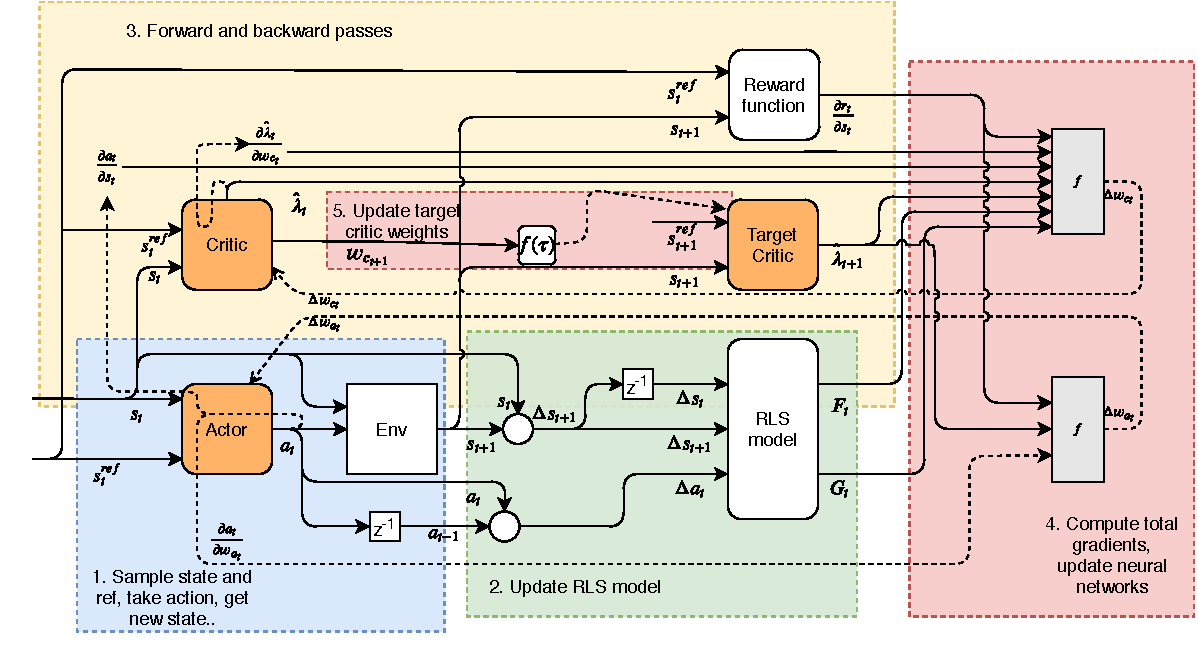
\includegraphics[width=\textwidth]{fig/2/flowchart.pdf}
    \caption{Flowchart of the information during a single complete time-step of the IDHP learning framework. Solid lines feed-forward information, while dashed lines indicate feed-back update paths. }
    \label{fig:idhp_flowchart}
\end{figure}

The structure of the IDHP agent is based on that first described in \cite{Zhou2018DHP} and expanded upon in \cite{Heyer2020}, and contains four main parametric structures: actor $\pi$, critic $\lambda$, target critic $\lambda'$, and an incremental model of the plant. Fig. \ref{fig:idhp_flowchart} shows how the components of the agent interact with the environment in a single timestep. The colored blocks represent parts of the agent while the white blocks are part of the environment. This section gives an overview of the different parts visible in this model. 

The original IDHP algorithm works forward in time, which requires predicting the states one timestep ahead. This has as an advantage that multiple updates can be done in every timestep, but also means that the accuracy is entirely dependent on the quality of the prediction. In this paper, a backward-in-time approach such as in \cite{Heyer2020, Enns2003a} is chosen. Though this means only a single update can take place every timestep, the high update frequency assumed for the incremental model as described in section \ref{ssec:neuralnetworks} and reduced reliance on forward prediction outweigh this loss.

\subsubsection{Actor and critic neural networks} \label{ssec:neuralnetworks}
In this paper, neural networks are chosen as the function approximator for the actor, critic, and target critic. Specifically, single-hidden-layer fully-connected multi-layered perceptrons (MLPs) are the structure of choice. They are easy to use with RL libraries such as Tensorflow and PyTorch, widely used in RL-for-flight-control literature \cite{Bertsekas2000, Enns2002, Enns2003a, Enns2003b, Ferrari2004, VanKampen2006, Prokhorov1995, Balakrishnan1996, Prokhorov1997, Zhou2016HDP, Zhou2018DHP, Heyer2020}, can theoretically approximate any function arbitrarily well \cite{Hornik1989}, and are differentiable. The critic estimates the partial derivative of the state-value function with respect to the states, while the actor provides a direct mapping between the current state and the action to take. Their structures are shown in Fig. \ref{fig:nn_structure}. The input of both network types is the same: a combination of their respective input states and tracking errors, which are further elaborated on in Section \ref{ssec:controllerdesign}. Both networks use a single hidden layer with ten neurons, using hyperbolic tangent activation functions. The output of the critic and target critic networks consists of a linear output layer with the same dimension as the input. The actor network has a single sigmoid output neuron, corresponding to the required input range of the helicopter model used as explained in Section \ref{ssec:helimodel}.

\begin{figure}[hb]
    \centering
    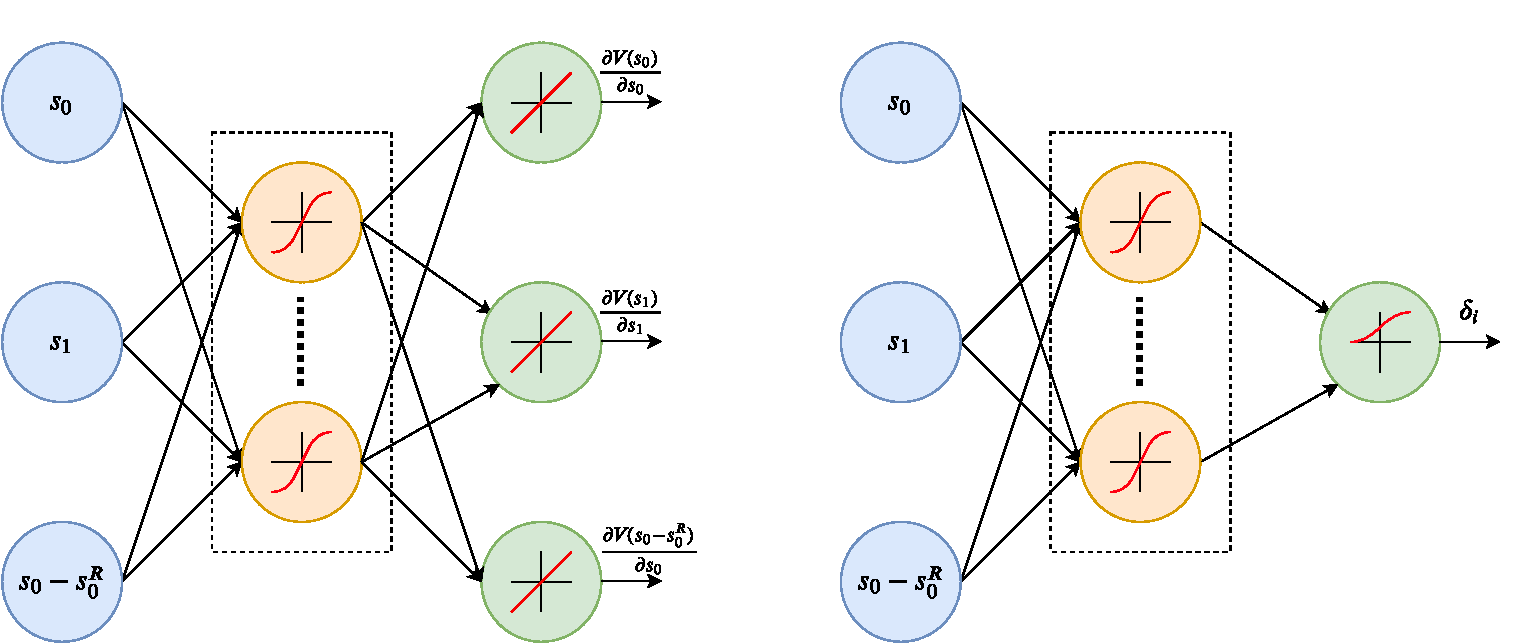
\includegraphics[width=\textwidth, trim={0 0 0.4cm 0.4cm}, clip]{fig/2/NNs2.pdf}
    \caption{Structure of the actor and critic neural networks. Both networks have a single hidden layer with ten neurons. }
    \label{fig:nn_structure}
\end{figure}

\subsubsection{Target critic}
A seperate target network as first introduced in \cite{Mnih2015, Lillicrap2015} is often used to stabilize learning in a Deep RL context by decoupling action selection and evaluation. This idea was successfully applied to IDHP in \cite{Heyer2020}, where it was shown that a separate target critic $\lambda'$ with weight vector $w_{c'}$ increased the stability of the learning process at the cost of learning speed. 

\subsubsection{Incremental model} \label{ssec:incrementalrls}
In contrast to older ADP methods, IDHP uses online estimation of an instantaneous linear model identified through Taylor expansion. Consider a discrete-time, nonlinear system $s_{t+1} = f(s_t, a_t)$. A Taylor expansion of this system around $t_0$ yields Eq. \eqref{eq:system_taylor}. By choosing the operating point to be $t_0 = t-1$, a number of new definitions can be made. 
Defining the partial derivatives of the state-transition function to be $F_t = \frac{\partial f(s_t, a_t) }{\partial s_t }$  (the system matrix) and $G_t = \frac{\partial f(s_t, a_t) }{\partial a_t}$ (the control matrix), as well as defining the state and control \textit{increments} to be $\Delta s_t = (s_t - s_{t-1})$ and $\Delta a_t = (a_t - a_{t-1})$, results in the incremental form of the Taylor expansion shown in Eq. \eqref{eq:system_incremental}. Given the assumption of a high sampling rate and slow dynamics, the incremental model form provides a valid linearized, time-varying approximation to the real nonlinear system \cite{Zhou2016iADP}.

\begin{equation}
\label{eq:system_taylor}
    s_{t+1} \approx f(s_{t_0}, a_{t_0}) + \frac{\partial f(s, a) }{\partial s } |_{s_{t_0}, a_{t_0}} (s_t - s_{t_0}) + \frac{\partial f(s, a) }{\partial a } |_{s_{t_0}, a_{t_0}} (a_t - a_{t_0})
\end{equation}
\begin{equation} \label{eq:system_incremental}
    \begin{split}
        s_{t+1} &\approx s_t + F_{t-1} (s_t - s_{t-1}) + G_{t-1} (a_t - a_{t-1}) \\
        \Delta s_{t+1} &= F_{t-1} \Delta s_t + G_{t-1} \Delta a_t
    \end{split}
\end{equation}

\subsubsection{Reward function} \label{ssec:rewardfunction}
In this paper, the reward is designed to be a negative, weighted, squared difference between the reference state and the new actual state, as defined in Eq. \eqref{eq:reward_definition}, with $P \in \mathbb{R}^{p \times n}$ the (Boolean) state selection matrix and $Q \in \mathbb{R}^{p \times p}$ the state weighting matrix. This definition provides the agent with a rich, informative reward signal at each timestep and is inherently differentiable, which is a requirement for the IDHP algorithm explained in section \ref{ssec:idhp}. The derivative of the reward function with respect to the state is given in Eq. \eqref{eq:reward_derivative}.

\begin{equation} \label{eq:reward_definition}
    r_{t+1} = -P\left(s_{t+1} - s_t^r\right)^T QP\left(s_{t+1} - s_t^r\right)
\end{equation}
\begin{equation} \label{eq:reward_derivative}
    \frac{\partial r_{t+1}}{\partial s_{t+1}} = -2P\left(s_{t+1} - s_t^r\right)^TQP
\end{equation}

\subsection{Update rules} \label{ssec:updaterules}
In this section, the update rules for the four parametric structures in the IDHP agent are described in the same order as in which they are updated in each timestep. For brevity, the reference state $s_t^r$, actor weight $w_a(t)$, critic weight $w_c(t)$, and target critic weight $w_{c'}(t)$ are not explicitly shown. Therefore, the four entities in Eq. \eqref{eq:shorthands} are interchangeable.

\begin{equation} \label{eq:shorthands}
    \lambda(s_t, s^R_t, w_c(t)) = \lambda(s_t) \qquad \lambda'(s_t, s^R_t, w_{c'}(t)) = \lambda'(s_t) \qquad \pi(s_t, s_t^R, w_a(t)) = \pi(s_t)
\end{equation}

\subsubsection{Incremental model}
The incremental model is identified through Recursive Least Squares (RLS) estimation. RLS is similar to a Kalman filter, making it very efficient in both computational and memory cost, and avoiding any potential problems with matrix inversions. The current state and control matrix are estimated together in one parameter matrix $\hat{\Theta}_t$, as shown in Eq. \eqref{eq:rls1}. 
\begin{equation} \label{eq:rls1}
    \hat{\Theta}_{t-1} = \begin{bmatrix} \hat{F}^T_{t-1} \\ \hat{G}^T_{t-1}\end{bmatrix}
\end{equation}
The parameter matrix is accompanied by a covariance matrix $P_t$, which provides an indication of the reliability of the parameter estimates. For the update process, first, a prediction of the next state increment, $\Delta \hat{s}_{t+1}$, is made using the current state and action increments as well as the current parameter matrix, as shown in Eqs. \eqref{eq:rls2} and \eqref{eq:rls3}. 
\begin{equation} \label{eq:rls2}
    X_t = \begin{bmatrix} \Delta s_t \\ \Delta a_t \end{bmatrix}
\end{equation}
\begin{equation} \label{eq:rls3}
    \Delta \hat{s}_{t+1} = \left(X_t^T \hat{\Theta}_{t-1}\right)^T
\end{equation}
This prediction is then compared with the actual state increment, and the prediction error, also known as innovation, is computed as $\epsilon_t = (\Delta s_{t+1} - \Delta \hat{s}_{t+1})^T$. Finally, the parameter and covariance matrices are updated according to Eqs. \eqref{eq:rls4} and \eqref{eq:rls5}, respectively, where $\kappa \in [0,1]$ is the scalar forgetting factor, which exponentially decays the importance of older measurements. 
\begin{equation} \label{eq:rls4}
    \hat{\Theta}_{t} = \hat{\Theta}_{t-1} + \frac{\hat{P}_{t-1} X_t \epsilon_t}{\kappa + X_t^T \hat{P}_{t-1} X_t}
\end{equation} 
\begin{equation} \label{eq:rls5}
    \hat{P}_t = \frac{1}{\kappa}\left[\hat{P}_{t-1} - \frac{\hat{P}_{t-1} X_t X_t^T \hat{P}_{t-1}}{\kappa + X_t^T \hat{P}_{t-1} X_t}\right]
\end{equation}

\subsubsection{Critic}
The critic in IDHP estimates the partial derivative of the state-value function with respect to the states: $\lambda(s_t, s^R_t) = \frac{\partial V(s_t, s^R_t)}{\partial s_t}$. The critic is updated by means of a one-step temporal difference (TD) backup operation that minimizes the mean-squared error of the critic error: $L_C = \frac{1}{2}e_c^2$. The critic error is the partial derivative of the one-step TD error with respect to the state vector as defined in Eq. \eqref{eq:critic_error}. 

\begin{equation} \label{eq:critic_error}
    \begin{split}
        e_c &= -\frac{\partial \left[ r(s_{t+1}, s^R_t) + \gamma V(s_{t+1}) - V(s_t) \right]}{ \partial s_t} \\
        &= -\left[\frac{\partial r(s_{t+1}, s^R_t)}{ \partial s_{t+1}} + \gamma \lambda'(s_{t+1}, s^R_{t+1})\right] \frac{\partial s_{t+1}}{\partial s_t } + \lambda(s_{t}, s^R_t)
    \end{split}
\end{equation}

The value of the next state $s_{t+1}$ is dependent on both the previous state and the action. Therefore, its derivative with respect to the previous state, which is the final term in Eq. \eqref{eq:critic_error}, must be expanded to contain both these pathways. The approximations to the new derivative terms, obtained previously from the RLS model, as well as the backpropagation result of the state through the actor network, can then be substituted to yield Eq. \eqref{eq:dst+1_ds}. 
\begin{equation} \label{eq:dst+1_ds}
\begin{split}
    \frac{\partial s_{t+1}}{\partial s_t } &= \frac{\partial f(s_t, a_t)}{\partial s_t } + \frac{\partial f(s_t, a_t)}{\partial a_t } \frac{\partial a_t}{\partial s_t} \\
    &= \hat{F}_{t-1} + \hat{G}_{t-1} \frac{\partial \pi(s_t, s^R_t, w_c)}{\partial s_t}
\end{split}
\end{equation}
Finally, the critic weights are updated through gradient descent on the critic loss, with learning rate $\eta_c$, as shown in Eqs. \eqref{eq:critic_update} and \eqref{eq:critic_update_2}.
\begin{equation} \label{eq:critic_update}
    w_c(t+1) = w_c(t) + \Delta w_c(t)
\end{equation}
\begin{equation} \label{eq:critic_update_2}
\begin{split}
    \Delta w_c(t) &= -\eta_c \frac{\partial L_C}{\partial w_c } =  -\eta_c \frac{\partial L_C}{\partial \lambda(s_{t}, s^R_t, w_c(t))} \frac{\partial \lambda(s_{t}, s^R_t, w_c(t))}{\partial w_c(t)} \\
    &= -\eta_c e_c(t) \frac{\partial \lambda(s_{t}, s^R_t, w_c(t))}{\partial w_c(t)}
\end{split}
\end{equation}

\subsubsection{Actor}
The goal of the actor is to find a policy which maximizes the state-value function: the optimal policy $\pi^*$. Consequently, the optimal action $a^*$ is defined as:
\begin{equation} \label{eq:optimalpolicy}
    a^*_t = \pi^*(s_t, s^R_t, w_a(t)) = arg \max_{a_t} V(s_t, s^R_t)
\end{equation}
Because the update takes place after a state transition, the TD(0) expansion of this value can be maximized instead. Consequently, the loss function to minimize with gradient descent is the negative TD(0) target, as shown in Eq. \eqref{eq:actorloss}.
\begin{equation} \label{eq:actorloss}
    L_A = -V(s_t, s^R_t) = -\left[ r(s_{t+1}, s^R_t) + \gamma V(s_{t+1}, s^R_{t+1}) \right]
\end{equation}
The state-value function is not directly dependent on the weights of the actor. Therefore, the update path takes place through the critic, reward function and environment model instead, as shown in Eq. \eqref{eq:actorlossderiv}.
\begin{equation} \label{eq:actorlossderiv}
\begin{split}
    \frac{\partial L_A}{\partial w_a} &= -\frac{\partial \left[ r(s_{t+1}, s^R_t) + \gamma V(s_{t+1}, s^R_{t+1}) \right]}{\partial a_t}\frac{\partial a_t}{\partial w_a } \\
    &= -\left[ \frac{\partial r_t}{\partial s_{t+1} } + \gamma \frac{\partial V(s_{t+1})}{\partial s_{t+1} } \right] \frac{\partial s_{t+1}}{\partial a_t } \frac{\partial a_t}{\partial w_a } \\
    &= -\left[ \frac{\partial r_t}{\partial s_{t+1} } + \gamma \lambda'(s_{t+1}) \right] G_{t-1} \frac{\partial \pi(s_t)}{\partial w_a }
\end{split}
\end{equation}

As with the critic, the actor weights are updated through gradient descent with learning rate $\eta_a$, as shown in Eq. \eqref{eq:actorupdate}.

\begin{equation} \label{eq:actorupdate}
    w_a(t+1) = w_a(t) + \Delta w_a(t) = w_a(t) - \eta_a \frac{\partial L_A}{\partial w_a}
\end{equation}

\subsubsection{Target critic}
Finally, the target critic is updated towards the critic using soft updates \cite{Lillicrap2015}, also known as Polyak averaging \cite{Lee2019}, as shown in Eq. \eqref{eq:targetcriticupdate}, where $\tau$ indicates the (usually small) mixing factor. 

\begin{equation} \label{eq:targetcriticupdate}
    w_{c'}(t+1) = \tau w_{c}(t+1) + (1-\tau) w_{c'}(t)
\end{equation}

% \frac{\partial }{\partial  } 
\section{Controller design} \label{sec:controller}
In this section, the design of the flight controller is discussed. First, the helicopter model used in the experiments is introduced. Afterwards, the proposed flight control architecture used to control this model is presented, and the most important hyperparameters are given.

\subsection{Helicopter model} \label{ssec:helimodel}

The helicopter model used is a nonlinear, six-degrees-of-freedom model of the Messerschmitt-Bölkow-Blohm (MBB) Bo 105 which was developed at the TU Delft \cite{Pavel1996, VanDerVorst1998} and subsequently modified with engine and rotor speed dynamics \cite{Gille2006}. The main rotor inflow is assumed to be uniform, with analytical blade element equations used for the forces and moments. The main rotor speed is dependant on the interplay between four sources of drag and the engine, the dynamics of which in turn are based on \cite{book:padfield} with reaction time modeled as a first-order lag. The tail rotor is modeled as an actuator disk, and linear aerodynamics are used to model the horizontal and vertical tails as well as the fuselage. The simulation model is run at 100Hz, assuming synchronous clean measurements and no turbulence. The state and action space of the model are given in Eq. \eqref{eq:heli_model_states} and Eq. \eqref{eq:heli_model_actions}.

\begin{equation} \label{eq:heli_model_states}
    s = \Big[u \enspace v \enspace w \enspace p \enspace q \enspace r \enspace \phi \enspace \theta\enspace \psi\enspace x\enspace y\enspace z\enspace \lambda_{0_{mr}}\enspace \lambda_{0_{tr}}\enspace \Omega \enspace P_{req}\enspace P_{av} \Big]^T
\end{equation}
\begin{equation} \label{eq:heli_model_actions}
    a = \begin{bmatrix} \delta_{col} & \delta_{lon} & \delta_{lat} & \delta_{ped} \end{bmatrix}^T
\end{equation}

Control inputs are given in percentages corresponding to how far that control input is between its minimum and maximum angle, with maximum being up or right, depending on the control channel. Because of phase lag inherent in rotorcraft, these control inputs do not correspond 1:1 with their respective control angles, as a certain degree of mixing occurs in the swashplate \cite{book:padfield}. The saturation limits of these control angles corresponding to 0\% and 100\% control input are given in Table \ref{tab:heli_control_ranges}. 

\begin{table}[ht]
    \centering
    \caption{Saturation limits of the control angles of the Bo 105 simulation model \cite{BO105DataSheet}}
    \label{tab:heli_control_ranges}
    \begin{tabular}{@{}lccc@{}}
    \toprule
    Control channel     & Symbol         & Associated control angle  & Saturation limits  \\ \midrule
    Collective          & $\delta_{col}$ & $\theta_0$        & [2, 18] deg   \\
    Longitudinal cyclic & $\delta_{lon}$ & $\theta_{1s}$     & [10, -5.5] deg \\
    Lateral cyclic      & $\delta_{lat}$ & $\theta_{1c}$     & [-6, 4] deg   \\
    Pedal               & $\delta_{ped}$ & $\theta_{0_{tr}}$ & [18, -6] deg  \\ \bottomrule
    \end{tabular}
\end{table}

\subsection{Flight controller} \label{ssec:controllerdesign}
The complete control system consists of a mixture of RL as well as conventional PID, and is shown in Fig. \ref{fig:controlsystem}. Only the longitudinal channels (collective and longitudinal cyclic) are controlled by the adaptive controllers, while the lateral channels (lateral cyclic and pedal) are controlled by conventional PID controllers. It must be noted that there is a strong degree of coupling between the different channels, and a unified controller would likely permit taking advantage of this in a way that multiple separate controllers cannot \cite{Enns2003a}. On the other hand, this set-up would also inevitably lead to slower learning, as it becomes inherently harder to learn the desired behavior of multiple coupled states from a scalar reward signal. Although there is a strong degree of coupling between the different channels, the controllers have distinct enough tasks to allow for decoupling of the controllers. The resulting agent input states and action vectors are shown in Eq. \eqref{eq:state_loncol}. The state-selection and weight matrices required to extract these states from the complete state are given in Eqs. \eqref{eq:matrices_col} and \eqref{eq:matrices_lon}. A lower value for $Q^{col}$ is chosen to bring the magnitudes of the rewards of both agents more in line with each other, allowing for easier tuning.

\begin{figure}[ht]
    \centering
    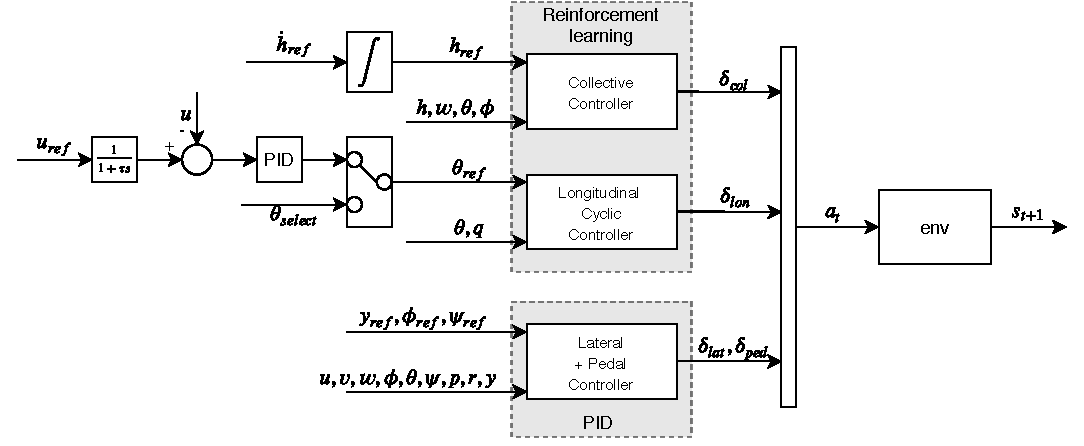
\includegraphics[width = 0.95\textwidth]{fig/3/controldiagram.pdf}
    \caption{High-level overview of the complete flight control system}
    \label{fig:controlsystem}
\end{figure}

\begin{equation} \label{eq:state_loncol}
    s^{col} = \begin{bmatrix} z & w & (z-z_{ref}) \end{bmatrix}^T \qquad s^{lon} = \begin{bmatrix} \theta & q & (\theta-\theta_{ref}) \end{bmatrix}^T
\end{equation}
\begin{equation} \label{eq:matrices_col}
    P^{col} = P^{lon} = \begin{bmatrix} 0 & 0 & 1 \end{bmatrix}
\end{equation}
\begin{equation} \label{eq:matrices_lon}
    Q^{col} = \begin{bmatrix} 0.1 \end{bmatrix} \quad Q^{lon} = \begin{bmatrix} 1 \end{bmatrix}
\end{equation}

\subsection{Hyperparameters} \label{ssec:hyperparameters}
The hyperparameters used by this implementation are shown in Table \ref{tab:hyperparams}. A number of these states have their values listed as *: these were determined empirically at first, but later fine-tuned by means a grid-search over multiple hyperparameter combinations as explained in Section \ref{ssec:trainingphase}. The others were determined empirically. The discount factor $\gamma$ is a measure of the importance of future rewards with respect to more immediate ones. A relatively large value of $\gamma$ is assumed in order to place a larger weight on the slow dynamics of the helicopter.

\begin{table}[h]
    \centering
    \caption{Hyperparameters for the IDHP agents. The values indicated with an asterix were fine-tuned in the first part of the experiment}
    \label{tab:hyperparams}
    \begin{tabular}{@{}lll@{}}
\toprule
Parameter                         & Description                                        & Value              \\ \midrule
$\gamma$                          & Discount factor                                    & 0.8*               \\
$\sigma_w$                        & NN weight initialization standard deviation        & 0.1*               \\
$\tau$                            & Target critic mixing factor                        & 0.01*              \\
$\eta^{lon}_{a} \; \eta^{lon}_c$  & Longitudinal agent actor and critic learning rates & 5*                 \\
$\eta^{col}_{a} \; \eta^{col}_c$  & Collective agent actor and critic learning rates                    & 0.1*               \\
$\kappa$                          & RLS estimator forgetting factor                    & 0.999              \\
$\hat{F}_0, \hat{G}_0, \hat{P}_0$ & Initial RLS matrices                               & $I, 0, I\cdot10^8$ \\ \bottomrule
\end{tabular}
\end{table} 
\section{Experiment} \label{sec:experiment}
As described in Section \ref{sec:controller}, only the longitudinal motions are controlled by reinforcement learning agents. This section explains the experiments performed to test the proposed control system in the longitudinal plane, while keeping lateral motions to a minimum. Throughout all phases, the lateral motion controller had the task of keeping the deviation in lateral path distance and heading angle at a minimum. This was done by supplying the lateral PID controller with the references shown in Eq. \eqref{eq:lateral_references}.
\begin{equation} \label{eq:lateral_references}
    y_{ref} = 0 \qquad \psi_{ref} = 0 \qquad \phi_{ref} = \phi_{trim}
\end{equation}

The experiment consisted of two phases: an (online) training phase and a test phase. The training phase consisted of two parts. First, a training scenario was designed that could reliably allow the reinforcement learning controller to converge while containing sufficiently aggressive manoeuvres for real scenarios. Next, the optimal training hyperparameters  for training were determined by means of a grid search over various hyperparameter combinations and random seeds. For the test phase, two manoeuvres were designed to push the limits of the newly trained controller. 

\subsection{Training phase} \label{ssec:trainingphase}

In the training phase, the RL controller is asked to perform basic control tasks of increasing difficulty in order to achieve a certain baseline performance. To that end, the cyclic and collective agents were trained semi-separated from each other for 120 seconds in total. The environment is initialized at level, low-speed cruise, $V_{tas} = 15\si[per-mode=symbol]{\meter \per \second}$. For the first 60 seconds, the cyclic is training while the collective is controlled by a PID controller that is tasked with keeping a constant altitude. In the second minute, the collective is actively trained while the cyclic fine-tunes. 

The reference signal is as follows. 
The cyclic controller follows a reference pitch angle of format shown in Eq. \eqref{eq:theta_ref}, while the collective controller follows a reference altitude created by numerically integrating a given vertical velocity. The complete flight profile is shown in Fig. \ref{fig:reference_training}. 
\begin{equation} \label{eq:theta_ref}
    \theta_{ref} = A_{ref} \frac{\pi}{180} \cdot \sin\left(\frac{2 \pi\cdot t}{10} \right)
\end{equation}

\begin{figure}[ht]
    \centering
    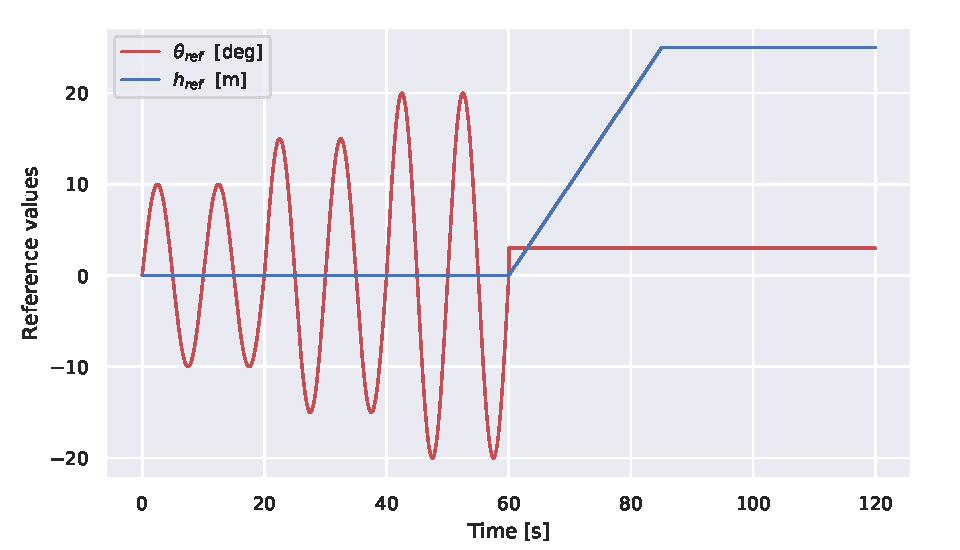
\includegraphics[width=0.9\textwidth]{fig/4/reference_training.pdf}
    \caption[]{Reference pitch angle and altitude during the training scenario}
    \label{fig:reference_training}
\end{figure}

It can be seen that the pitch angle reference signal amplitude $A_{ref}$ increases in steps over the first minute of training time, starting at $10\si{\degree}$, increasing to $15\si{\degree}$ after 20 seconds, and $20\si{\degree}$ after 40 seconds. This approach was found to lower the chance of the agent overshooting the reference significantly when provided with a very large tracking error early in training.
After 60 seconds, the learning rate of the cyclic agent is reduced by 90\%, the collective PID controller is switched off, and the collective RL agent starts training. The learning task of the collective agent is a steady climb with a climb rate of 2$\si[per-mode=symbol]{\meter \per \second}$ for 30 seconds, followed by an altitude hold for 30 seconds. Meanwhile, the cyclic is asked for a constant pitch angle $\theta_{ref} = 2.5\si{\degree}$ to steadily reduce forward airspeed. At the end of the training run, the helicopter should be at steady altitude and approximately zero airspeed. 

To help with the incremental model identification, an exponentially decaying sinusoidal excitation is applied to both inputs in the first eight seconds. A sine signal was preferred over other common excitation patterns such as 3211 or doublet because it exposes the model to different action increments as well as different state increments each timestep, allowing for more rapid convergence. 

The optimal hyperparameters for training were found by means of a grid search. Each combination of parameters was tested for 100 trials, and the success rate and final performance of each experiment was measured. The final performance is measured in the root-mean-squared error (RMSE) of the final 10 seconds of the experiment. Those hyperparameters with the best combination of success rate and final performance were used to train one agent whose weights were then saved and used as a starting point for the manoeuvres in the test phase.

\subsection{Test phase} \label{ssec:testphase}

The test phase consisted of two manoeuvres aimed at pushing different parts of the longitudinal envelope. Both manoeuvres are initialized from a pre-trained agent, but with 90\% reduced learning rates with respect to the training scenario. 

The first manoeuvre was a modified ADS-33 \cite{ADS33} acceleration-deceleration. Its objective is to check the heave and pitch axis for aggressive manoeuvring near the rotorcraft limits of performance, undesirable longitudinal-lateral coupling, and harmony between the pitch and heave controls. The desired performance characteristics are as follows. From hover, the aircraft accelerates to $25\si[per-mode=symbol]{\meter \per \second}$ using maximum power while maintaining altitude and lateral track deviations below 15 and 3 meters, respectively. After attaining the target speed, an immediate deceleration takes place, achieving at least $30\si{\degree}$ pitch-up attitude and less than 5\% engine power. 

The second manoeuvre was a one-engine inoperative landing based on \cite{Gille2006}. This manoeuvre checked the controller for the ability to quickly adapt to a new trim point, perform steady flight for a while, followed by an immediate aggressive manoeuvre under reduced engine power. A single engine failure occured at low altitude, after which the helicopter no longer had enough power to perform a balked landing. Therefore a continuous landing with flare manoeuvre was performed. The safe limits of forward and downward velocity during touchdown, $u_{max}$ and $w_{max}$, were assumed to be 4.5$\si[per-mode=symbol]{\meter \per \second}$ and 1.5$\si[per-mode=symbol]{\meter \per \second}$, respectively \cite{OEILandings}.
\section{Results}\label{sec:results}
As described before, the experiment consisted of two phases, with three parts in total: the design of a training scenario, a grid search over the best hyperparameters, and the manoeuvres flown by the resulting controller. Although the training scenario design took place first, the resulting parameters came out of the settings found with the grid search. Therefore, this section presents the results of the three different experiment phases presented above in a slightly different order. First, the results of the hyperparameter search are presented. Those hyperparameters with the best performance were then used as a starting point for the training phase. Finally, the controller that was resulted from the training phase was saved, and the two test manoeuvres were performed by starting from the training save point. 

\subsection{Hyperparameter search} \label{ssec:results:training}
The grid search over the hyperparameters yielded two sets of results. Firstly, the success rate, defined as the percentage of trials that did not end prematurely, is shown in Fig. \ref{fig:training_params_success}. Trials could end prematurely in two ways: either by breaking the performance limits of $\pm90\si{\degree}$ in pitch and roll, or by "parameter explosion", which is numerical overflow of the neural network weights. Secondly, the final performance of the successful runs, measured in RMSE in the final ten seconds of successful trials, is shown in Fig. \ref{fig:training_params_rms}. 

\begin{figure}[th]
    \centering
    \subfloat[Success rates]{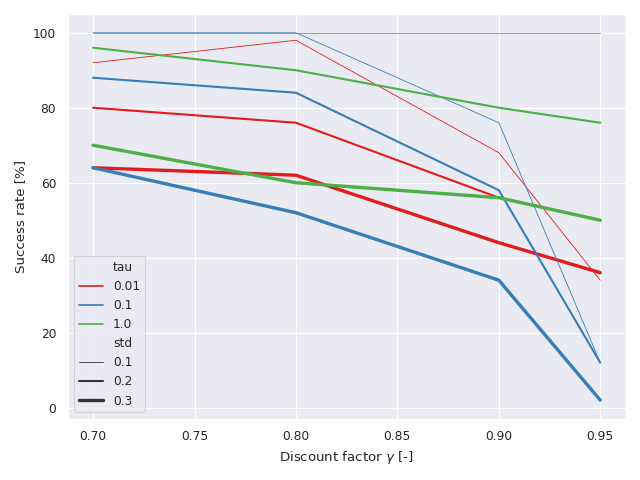
\includegraphics[width=0.45\textwidth]{fig/5/training/params_success.png} \label{fig:training_params_success}}
    \subfloat[Final performance]{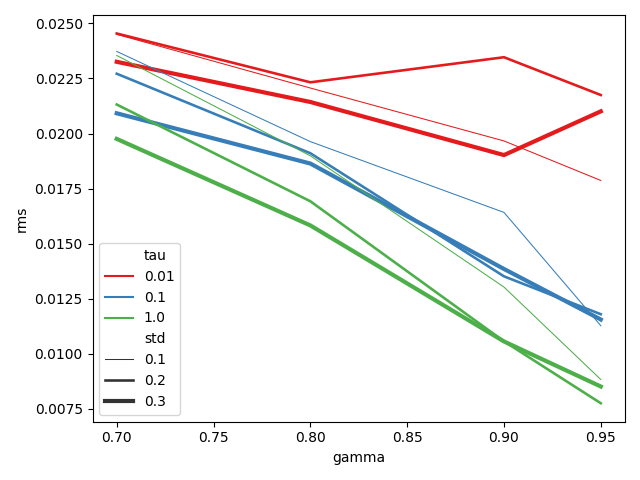
\includegraphics[width=0.45\textwidth]{fig/5/training/params_rms.png} \label{fig:training_params_rms}}
    \caption{Aggregated success rates and final performance of different combinations of training hyperparameters}
\end{figure}

Inspecting these figures, a few trends become visible. First, it can be seen that the discount factor $\gamma$ is simultaneously correlated with a lower success rate as well as higher final performance. This result exposes the "dual role" of the discount factor $\gamma$. As a discount factor explicitly weighs future rewards more or less strongly, it also implicitly serves as a variance reduction parameter, weighing the importance of the critic's estimate of value derivatives in the actor update. This makes a set-up with a low value of $\gamma$ less prone to the parameter explosion failure mode often found in ADP. On the other hand, a high value of $\gamma$ leads to stronger weighting of future rewards, which is important in tasks with relatively slow controls such as helicopter control. 
Secondly, in this implementation, higher values of $\tau$ were found to be correlated with both higher success rates and better final performance, all the way up to $\tau=1$. At $\tau=1$ the target critic immediately tracks the critic, and such is not used at all. This can be attributed to the fact that in this online learning scenario, the slow learning in presence of a target critic can actually cause the unstable helicopter environment to diverge more quickly than using a less robust but faster implementation without a target critic can. This was verified by comparing the failure modes with and without target critic: it was found that the majority of failures with a target critic in place were loss-of-control failures, while this shifted to numerical overflow failures when no target critic was in place. 
Thirdly, lower values of $\sigma_w$ were generally associated with higher success rates, but lower final performance. Based on these results, the hyperparameters used for training are shown in Fig. \ref{tab:training_end_hyperparams}. This combination showed a 100\% success rate in training over 100 random seeds while also having near-optimal final performance. 

\begin{table}[ht!]
\centering
\caption{Hyperparameters of the IDHP agents used in training}
\label{tab:training_end_hyperparams}
\begin{tabular}{@{}lll@{}}
\toprule
Hyperparameter               & Description                                 & Value \\ \midrule
$\gamma$                     & Discount factor                             & 0.95   \\
$\sigma_w$                   & Weight initialization standard deviation & 0.1   \\
$\tau$                       & Target critic mixing factor                 & 1.0  \\
$\eta^{lon}_{a} \; \eta^{lon}_c$ & Longitudinal agent actor and critic learning rates           & 5     \\
$\eta^{col}_{a} \; \eta^{col}_c $ & Collective agent learning rates             & 0.1   \\ \bottomrule
\end{tabular}
\end{table}

\subsection{Training phase}
A sample training episode is shown in Fig. \ref{fig:training_results}. It can be seen that both cyclic and collective are able to follow the reference signal after approximately ten seconds, after which the performance is slowly improved over the next 50 seconds. Around $t=90\si{\second}$, some yawing motion appears as the result of tail rotor saturation, which in return is the result of the collective approaching 90\% in low-speed flight. In the collective controller, it can be seen that manages to achieve two different steady-state (trim) points: even though the controller was initialized at the trim for 15$\si[per-mode=symbol]{\meter \per \second}$, it has no problem holding altitude at flight speeds as low as 2$\si[per-mode=symbol]{\meter \per \second}$.

\begin{figure}[htb!]
    \centering
    \subfloat[Tracking performance, control inputs and angular rates]{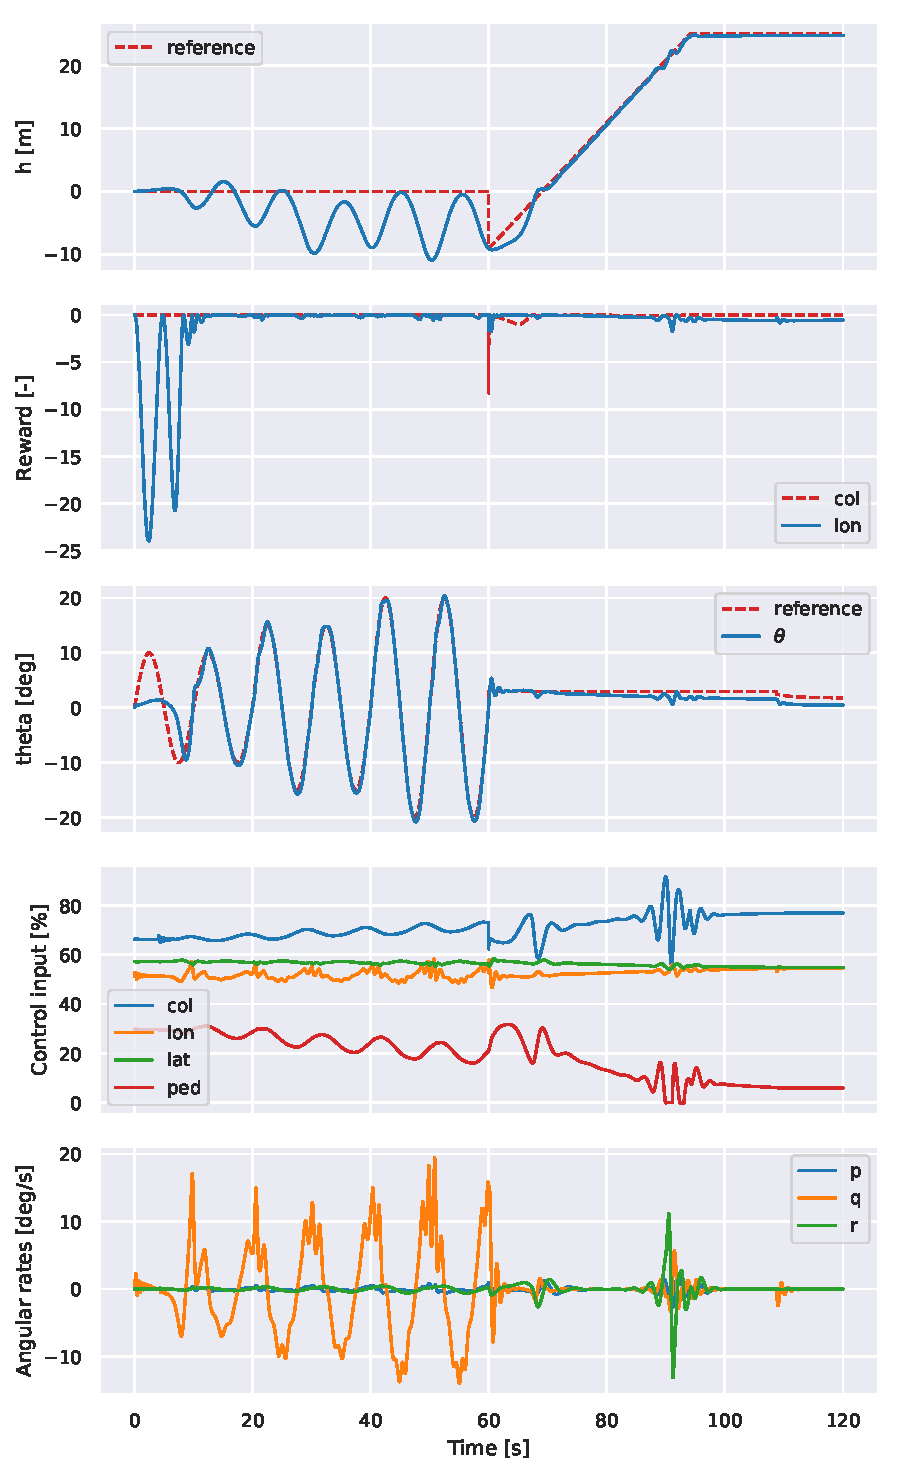
\includegraphics[width=0.48\textwidth]{fig/5/training/tracking.pdf} \label{fig:training_tracking}}
    \subfloat[Remaining state variables]{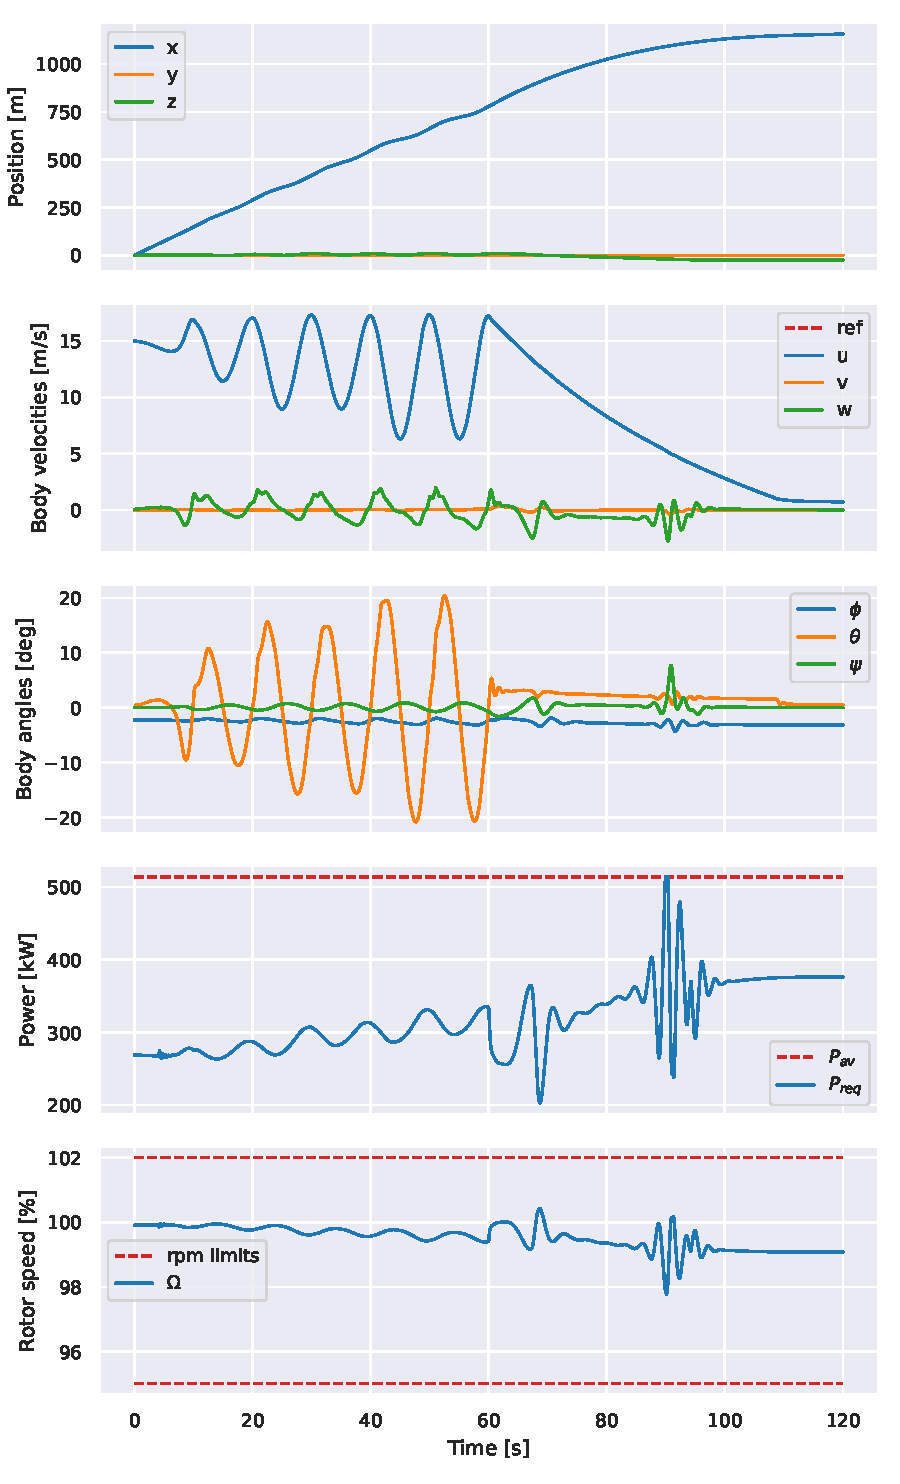
\includegraphics[width=0.48\textwidth]{fig/5/training/states.pdf} \label{fig:training_states}}
    \caption{Results of a sample training run}
    \label{fig:training_results}
\end{figure}

In Fig. \ref{fig:training_weights}, the learned parameters of the online estimated state and input matrices as well as the weights of both the actor and critic are shown. It can be seen that the parameters of both the state and input matrix in the incremental model converge within seconds, providing critical information to the actor and critic updates. 

\begin{figure}[htb]
    \centering
    \subfloat[Cyclic agent]{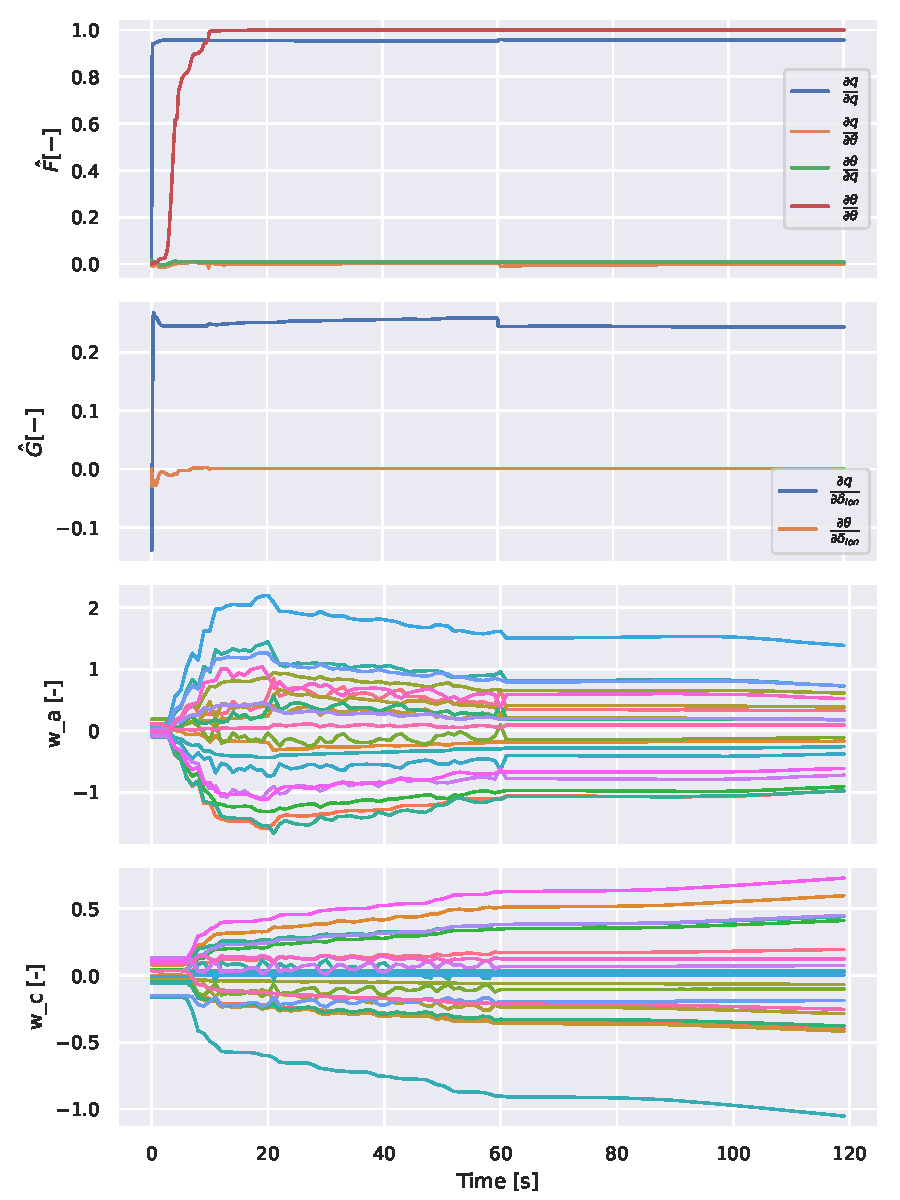
\includegraphics[width=0.48\textwidth]{fig/5/training/weights_cyclic.pdf} \label{fig:training_w_cyclic}}
    \subfloat[Collective agent]{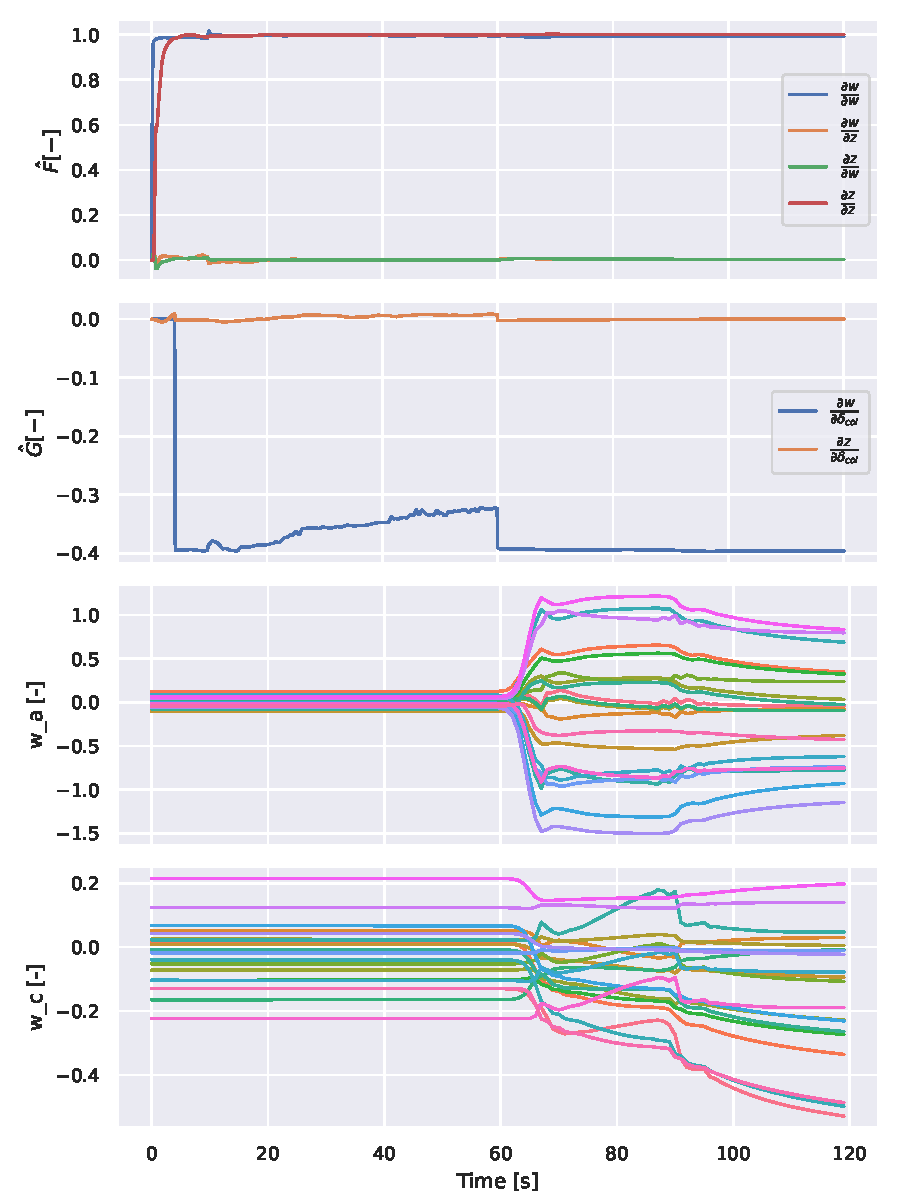
\includegraphics[width=0.48\textwidth]{fig/5/training/weights_collective.pdf} \label{fig:training_w_collective}}
    \caption{Estimates of the online identified incremental model, actor weights and critic weights during a sample training trial}
    \label{fig:training_weights}
\end{figure}

\subsection{Test phase} \label{ssec:results:test}
\subsubsection{Acceleration-deceleration}
% TODO: move legend in figure, add vertical lines  for flight phases
Fig. \ref{fig:results_acceldecel} shows the results of a successful episode from the proposed acceleration-deceleration test. In the figure, the different flight phases are indicated with numbered dashed vertical lines (NOTE NOT YET DONE). 
In phase 1, the helicopter is in hover. Some minor control excitation can be seen in the first second of the episode, as the environment in initialized in a slightly different state from saved agent. 

In phase 2, the helicopter starts accelerating from hover to $u=25\si[per-mode=symbol]{\meter \per \second}$. It can be seen that the actual forward velocity lags behind the commanded value quite significantly. The pitch angle reference is followed sharply in the sharp transient part of this phase, but is slightly above the reference during the second half of this phase. A slight altitude gain is also observed, though this is well within the limits of 15m. As a result of the high collective required for the acceleration, the pedal control saturates, leading to a slight yawing motion around $t = 8 \si{\second}$, which was the limiting factor in the aggressiveness of the manoeuvre. 

As soon at the required velocity is achieved, phase 3 starts and an aggressive pitch-up is performed to decelerate the helicopter. The leads to a sudden increase in altitude due to two reasons. Firstly, as the fuselage rotates from slightly pitched-down through the neutral position, the increases the vertical component of the thrust vector. Secondly, part of the lost kinetic energy of the helicopter is transferred to the main rotor, increasing the rotor speed to slightly below the maximum safe speed, which in turn increases the total thrust force. As a reaction to this, the collective is reduced significantly and the engine power is reduced to less than 5\%. The control system remains stable even with pitch rates over $40\si[per-mode=symbol]{\degree \per \second}$. The maximum pitch-up attitude of $24\si{\degree}$ is reached two seconds into the third phase. 

Throughout the episode, it can be observed that the reference pitch angle is smoothly tracked. The pitch angle does not reach the required $30\si{\degree}$ in the deceleration phase, as this would have led to large heading deviations due to pedal saturation. The maximum deviations in altitude, lateral track, and heading angle remain well within the performance bounds. 

The acceleration-deceleration did not meet all the desired performance standards of the ADS-33, as it was largely held back by collective-pedal coupling. This is likely a result of deficiencies in the helicopter model, which is rather simple. Similar trends were observed in \cite{VanDerVorst2001}. When compared to real-life test data, the trends of the control inputs were similar but the magnitude of the collective required was significantly smaller. 

\begin{figure}[htb]
    \centering
    \subfloat[Tracking performance, control inputs and angular rates]{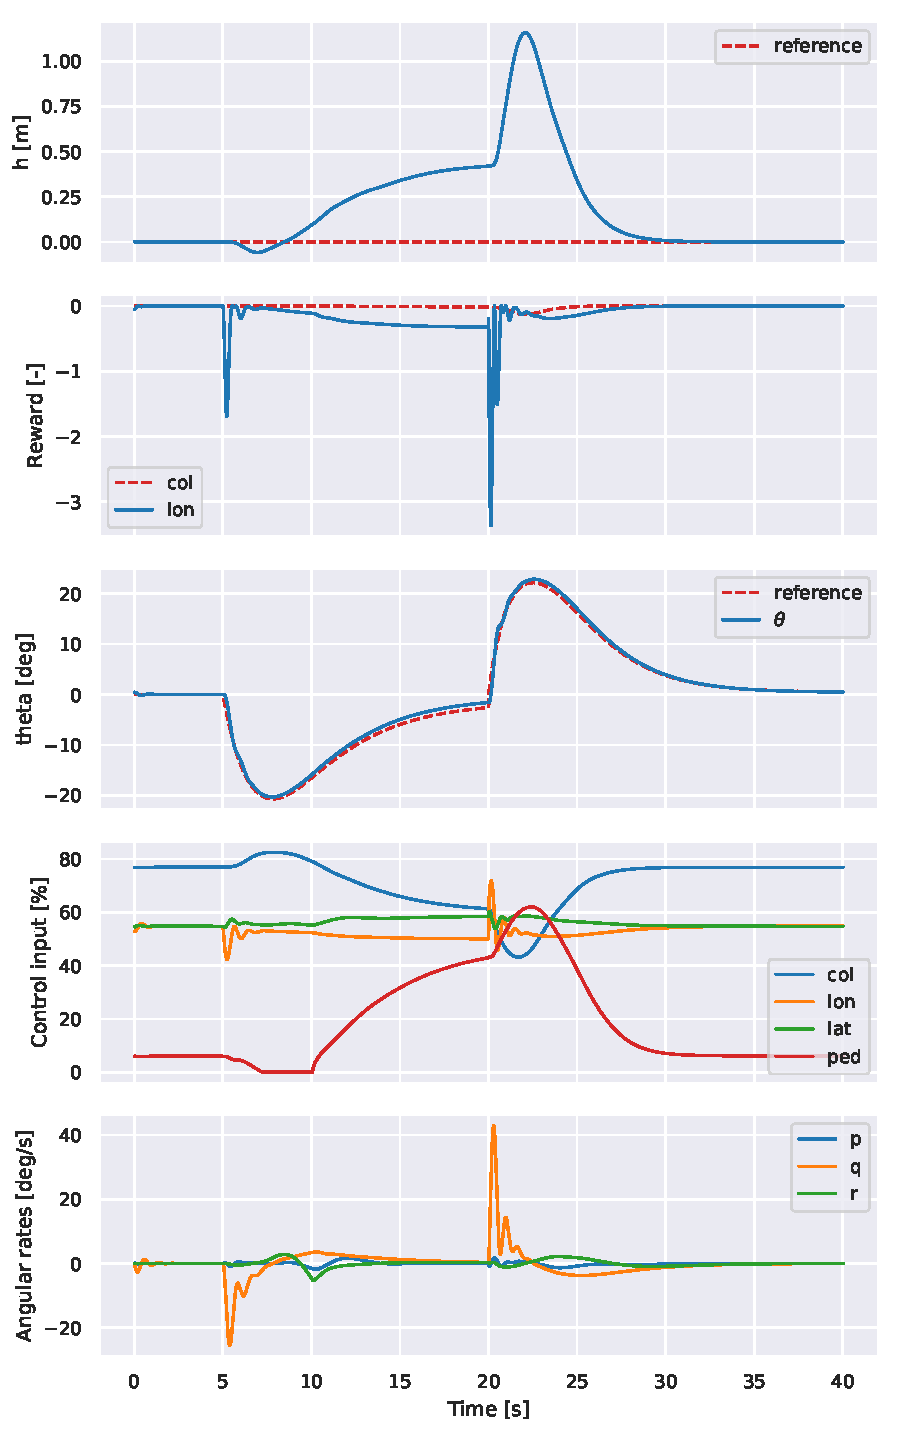
\includegraphics[width=0.48\textwidth]{fig/5/test/acdc/tracking.pdf} \label{fig:acdc_tracking}}
    \subfloat[Remaining state variables]{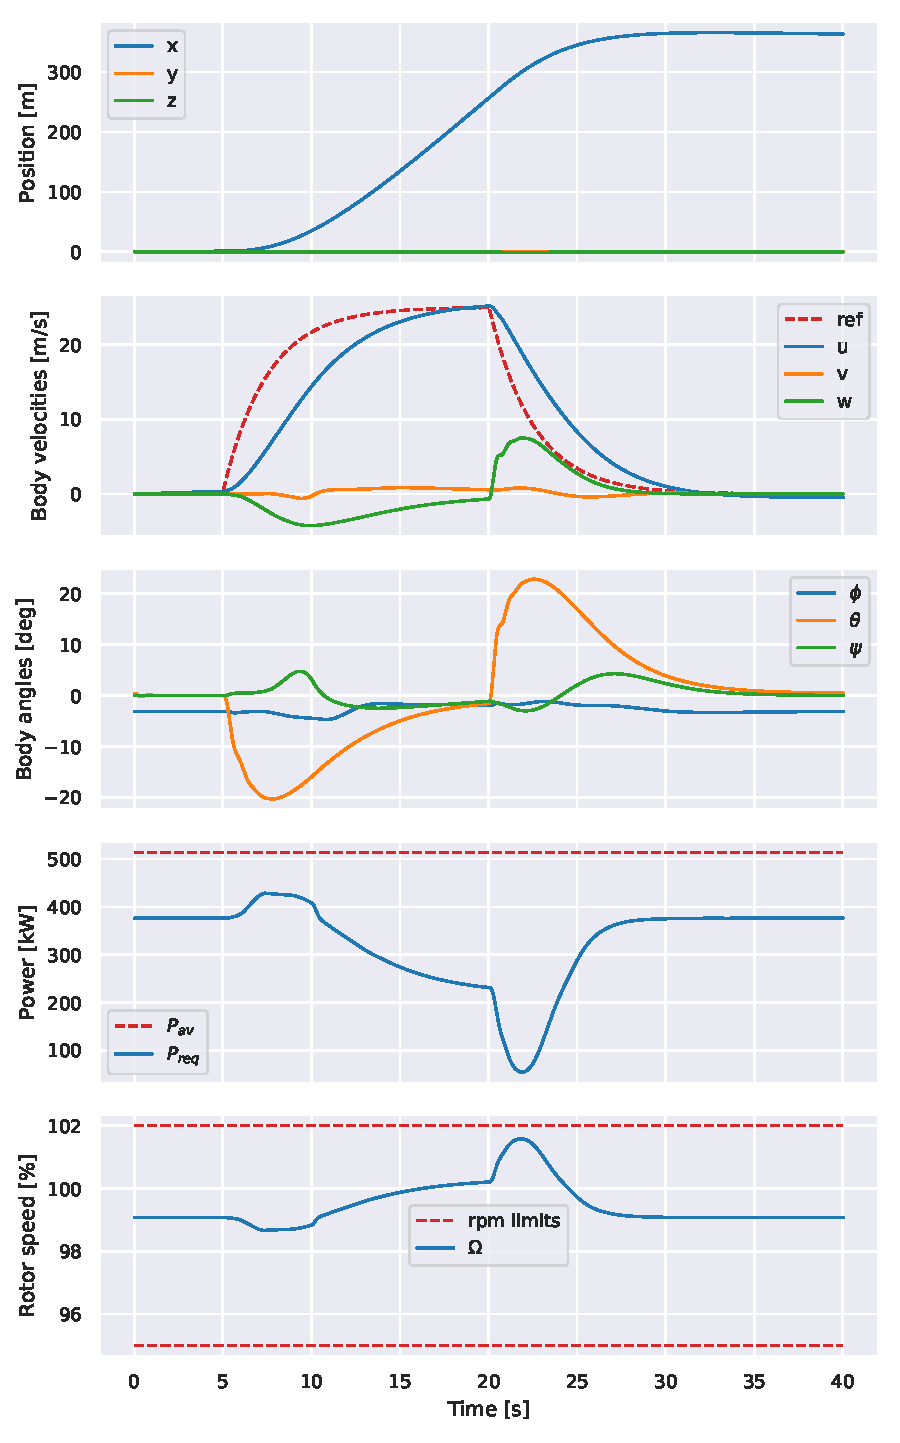
\includegraphics[width=0.48\textwidth]{fig/5/test/acdc/states.pdf} \label{fig:acdc_states}}
    \caption{Results of a sample run for the acceleration-deceleration test}
    \label{fig:results_acceldecel}
\end{figure}


\subsubsection{Continued landing}
The results of the continued landing test are shown in Fig. \ref{fig:results_landing}. 

In phase 1, a steady descending flight at a total airspeed of $V_{tas}=18\si[per-mode=symbol]{\meter \per \second}$ and a flight path angle $\gamma = -6\si{\degree}$ is performed. The agent, which was saved at approximately hover conditions, thus has to quickly establish a new approximate trim point. 

Phase 2 starts at $t=10\si{\second}$ when a single engine failure occurs, reducing the power available from the two-engine continuous limit $P_{aeo} = 514\si{\kilo\watt}$ to the single-engine transient limit $P_{oei,tr}=327\si{\kilo\watt}$. With a single engine the helicopter no longer has enough power to stop in a hover, requiring the performance of a continuous landing. However, in this steady descent phase, the engine is not performing at its limits, so nothing happens yet.

In phase 3, a flare is performed to reduce the forward airspeed as much as possible. The pitch angle reaches $17.6\si{\degree}$ when approximately $5\si{\meter}$ above the ground. To prevent the helicopter from losing too much altitude, the collective is also slightly increased while the forward airspeed is decreasing. The collective is then lowered and immediately increased to set in a slow descent with a reference vertical speed of $\dot{h}_{ref}=-0.5\si[per-mode=symbol]{\meter \per \second}$, while the cyclic is reduced to level out the airframe. As the forward airspeed decreases, the helicopter ends up in more and more of its own downwash, decreasing the efficiency and requiring more collective to keep the descent vertical speed stable. 

Phase 4 starts when the engine power reaches its maximum. As the engine power is insufficient to keep the descent steady, the collective is increased even further to trade rotor rotational speed for kinetic energy and cushion the last part of the landing. As a result, the helicopter touches down with forward and downward speeds of $u=3.11\si[per-mode=symbol]{\meter \per \second}$ and $w=0.82\si[per-mode=symbol]{\meter \per \second}$, which are both well within the safe values of 4.5$\si[per-mode=symbol]{\meter \per \second}$ and 1.5$\si[per-mode=symbol]{\meter \per \second}$, respectively. As the fourth phase lasted under five seconds, the choice for transient max power is warranted. Interestingly, it should be noted that the available power is likely underestimated as the ground effect is not taken into account in the simulation model. This would have increased the power available at these low speeds and altitudes, reducing the amount of rotor energy needed to cushion the landing. 

\begin{figure}[htb!]
    \centering
    \subfloat[Tracking performance, control inputs and angular rates]{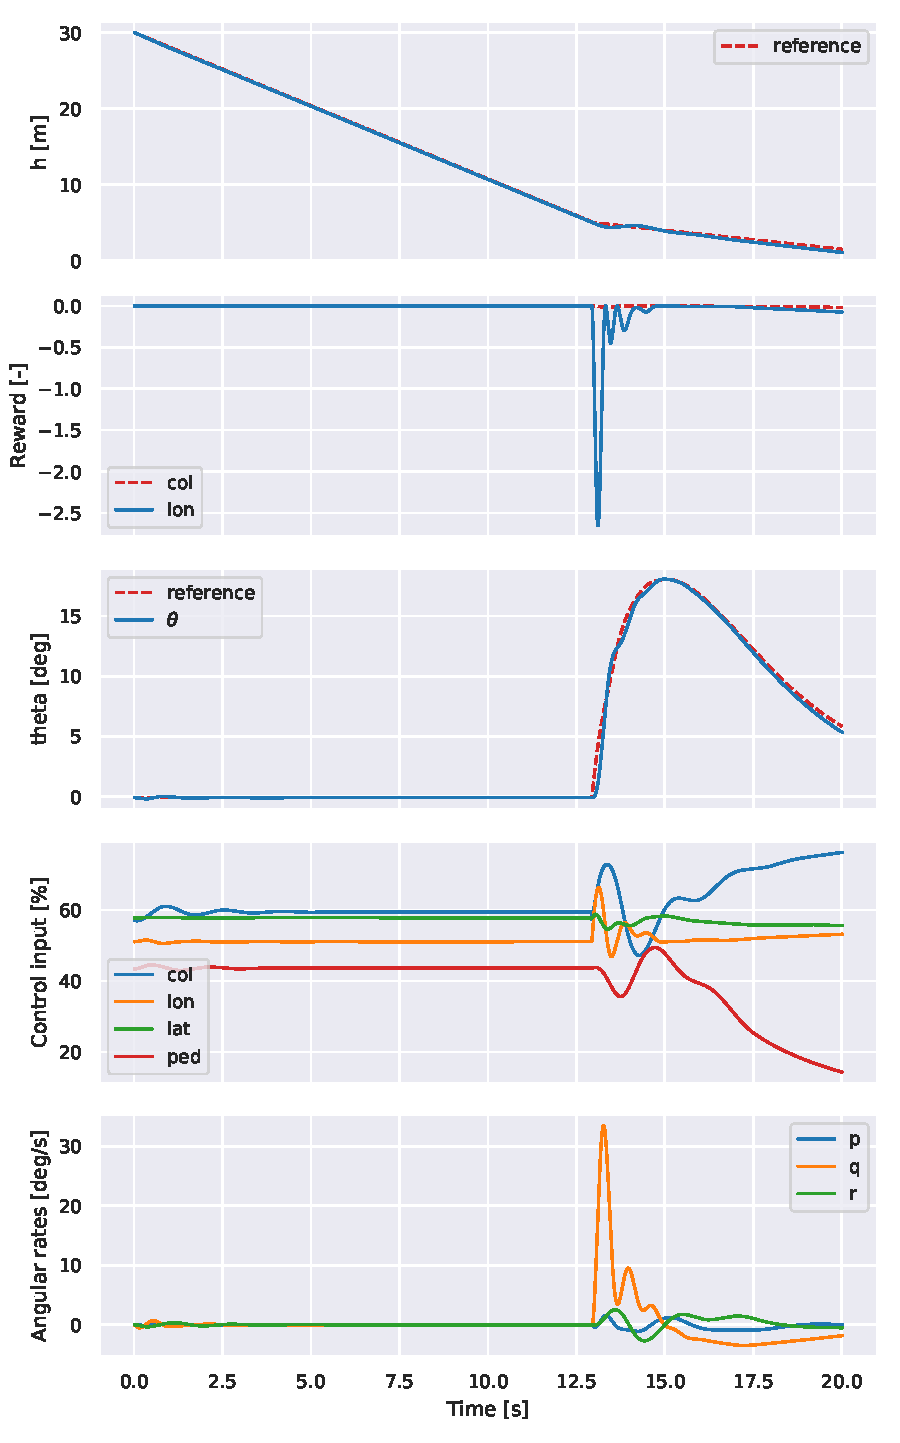
\includegraphics[width=0.48\textwidth]{fig/5/test/landing/tracking.pdf} \label{fig:land_tracking}}
    \subfloat[Remaining state variables]{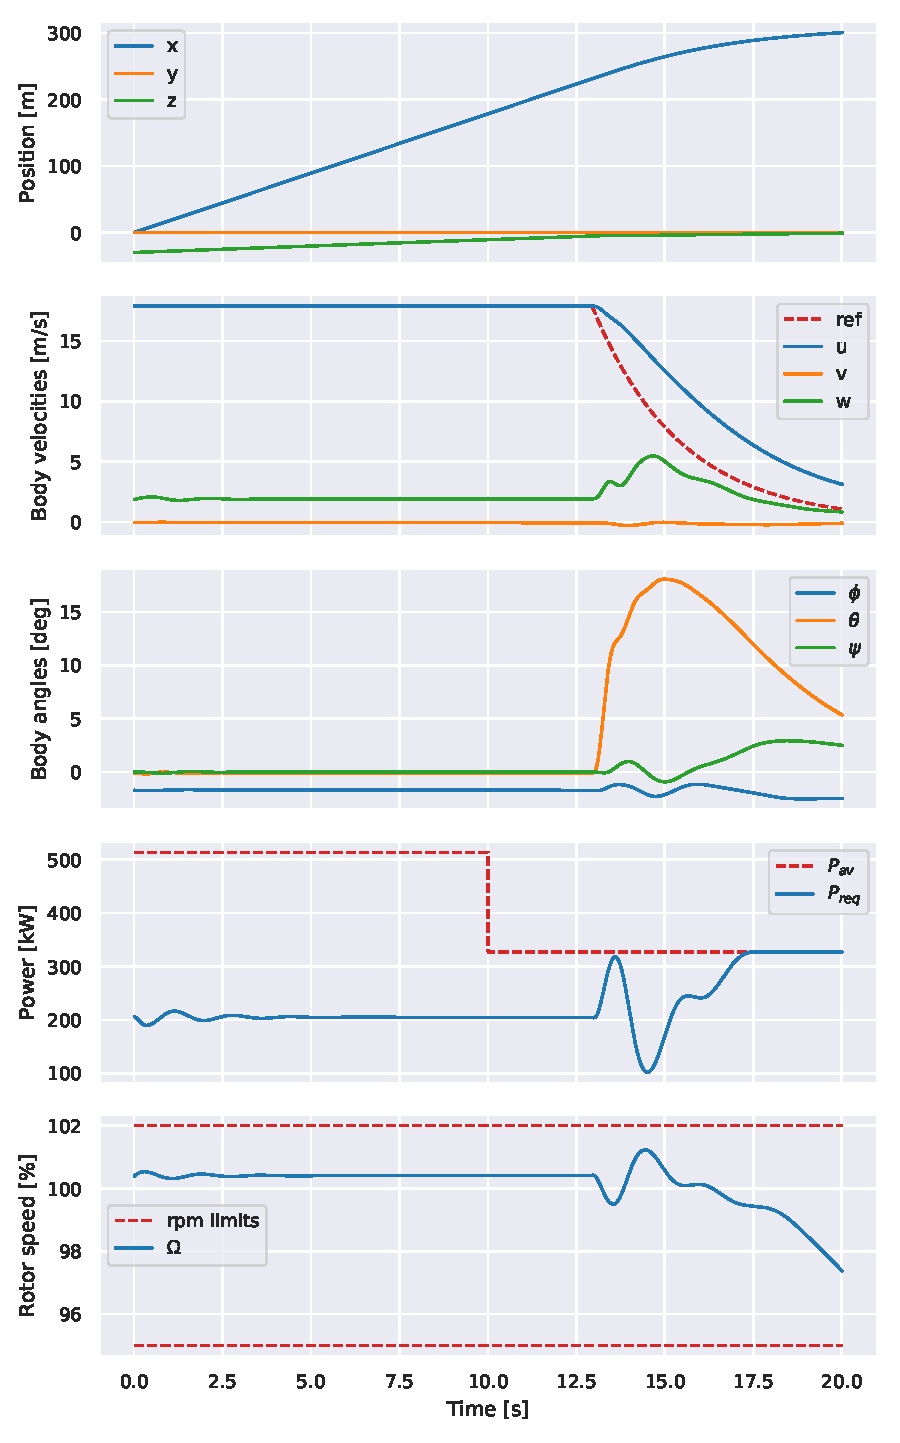
\includegraphics[width=0.48\textwidth]{fig/5/test/landing/states.pdf} \label{fig:land_states}}
    \caption{Results of a sample run for the landing test}
    \label{fig:results_landing}
\end{figure}

\FloatBarrier 
\section{Conclusion and Recommendations}\label{sec:conclusions}
The design and analysis of an IDHP-based flight controller for a Bo-105 helicopter are presented. The controller was shown to be able to reliably learn to directly control the pitch angle and altitude without an offline learning phase. Furthermore, the controller does not depend on any prior knowledge of the controlled system, and could therefore adapt to changes online. Results from \cite{Heyer2020}, indicating that the addition of a target critic is a valuable addition to the IDHP framework, were shown not to necessarily apply in all situations. Though a target critic adds learning stability, this is offset by the reduced learning speed, leading to frequent loss-of-control due to the inherent dynamic instability of rotorcraft. After a 120 second online training phase, the resulting controller was shown to be able to perform two different, aggressive maneuvers when provided with a proper reference signal. It can be concluded that the proposed framework is a first step towards a helicopter flight control system based on online reinforcement learning.

To further advance this field, further research is recommended. Firstly, the control system should be expanded to control all four axes instead of only the longitudinal motions. Although it was not found in this research, it is also speculated that a modification of the current setup where multiple control inputs are controlled by one agent could improve the performance of the control system.  The desired performance characteristics of the ADS-33 acceleration-deceleration manoeuvre could not be achieved because of unwanted collective-pedal coupling effects which are suggested to be due to modeling deficiencies. Therefore, the use of a higher-fidelity helicopter model with more degrees of freedom is suggested. Finally, the assumptions of clean measurements and no turbulence done in this research are not realistic. Future research should work on quantifying the effects of these two disturbances.  

\FloatBarrier
\bibliography{bibliography}

\end{document}
